% Options for packages loaded elsewhere
\PassOptionsToPackage{unicode}{hyperref}
\PassOptionsToPackage{hyphens}{url}
%
\documentclass[
]{article}
\usepackage{amsmath,amssymb}
\usepackage{lmodern}
\usepackage{iftex}
\ifPDFTeX
  \usepackage[T1]{fontenc}
  \usepackage[utf8]{inputenc}
  \usepackage{textcomp} % provide euro and other symbols
\else % if luatex or xetex
  \usepackage{unicode-math}
  \defaultfontfeatures{Scale=MatchLowercase}
  \defaultfontfeatures[\rmfamily]{Ligatures=TeX,Scale=1}
\fi
% Use upquote if available, for straight quotes in verbatim environments
\IfFileExists{upquote.sty}{\usepackage{upquote}}{}
\IfFileExists{microtype.sty}{% use microtype if available
  \usepackage[]{microtype}
  \UseMicrotypeSet[protrusion]{basicmath} % disable protrusion for tt fonts
}{}
\makeatletter
\@ifundefined{KOMAClassName}{% if non-KOMA class
  \IfFileExists{parskip.sty}{%
    \usepackage{parskip}
  }{% else
    \setlength{\parindent}{0pt}
    \setlength{\parskip}{6pt plus 2pt minus 1pt}}
}{% if KOMA class
  \KOMAoptions{parskip=half}}
\makeatother
\usepackage{xcolor}
\usepackage[margin=1in]{geometry}
\usepackage{color}
\usepackage{fancyvrb}
\newcommand{\VerbBar}{|}
\newcommand{\VERB}{\Verb[commandchars=\\\{\}]}
\DefineVerbatimEnvironment{Highlighting}{Verbatim}{commandchars=\\\{\}}
% Add ',fontsize=\small' for more characters per line
\usepackage{framed}
\definecolor{shadecolor}{RGB}{248,248,248}
\newenvironment{Shaded}{\begin{snugshade}}{\end{snugshade}}
\newcommand{\AlertTok}[1]{\textcolor[rgb]{0.94,0.16,0.16}{#1}}
\newcommand{\AnnotationTok}[1]{\textcolor[rgb]{0.56,0.35,0.01}{\textbf{\textit{#1}}}}
\newcommand{\AttributeTok}[1]{\textcolor[rgb]{0.77,0.63,0.00}{#1}}
\newcommand{\BaseNTok}[1]{\textcolor[rgb]{0.00,0.00,0.81}{#1}}
\newcommand{\BuiltInTok}[1]{#1}
\newcommand{\CharTok}[1]{\textcolor[rgb]{0.31,0.60,0.02}{#1}}
\newcommand{\CommentTok}[1]{\textcolor[rgb]{0.56,0.35,0.01}{\textit{#1}}}
\newcommand{\CommentVarTok}[1]{\textcolor[rgb]{0.56,0.35,0.01}{\textbf{\textit{#1}}}}
\newcommand{\ConstantTok}[1]{\textcolor[rgb]{0.00,0.00,0.00}{#1}}
\newcommand{\ControlFlowTok}[1]{\textcolor[rgb]{0.13,0.29,0.53}{\textbf{#1}}}
\newcommand{\DataTypeTok}[1]{\textcolor[rgb]{0.13,0.29,0.53}{#1}}
\newcommand{\DecValTok}[1]{\textcolor[rgb]{0.00,0.00,0.81}{#1}}
\newcommand{\DocumentationTok}[1]{\textcolor[rgb]{0.56,0.35,0.01}{\textbf{\textit{#1}}}}
\newcommand{\ErrorTok}[1]{\textcolor[rgb]{0.64,0.00,0.00}{\textbf{#1}}}
\newcommand{\ExtensionTok}[1]{#1}
\newcommand{\FloatTok}[1]{\textcolor[rgb]{0.00,0.00,0.81}{#1}}
\newcommand{\FunctionTok}[1]{\textcolor[rgb]{0.00,0.00,0.00}{#1}}
\newcommand{\ImportTok}[1]{#1}
\newcommand{\InformationTok}[1]{\textcolor[rgb]{0.56,0.35,0.01}{\textbf{\textit{#1}}}}
\newcommand{\KeywordTok}[1]{\textcolor[rgb]{0.13,0.29,0.53}{\textbf{#1}}}
\newcommand{\NormalTok}[1]{#1}
\newcommand{\OperatorTok}[1]{\textcolor[rgb]{0.81,0.36,0.00}{\textbf{#1}}}
\newcommand{\OtherTok}[1]{\textcolor[rgb]{0.56,0.35,0.01}{#1}}
\newcommand{\PreprocessorTok}[1]{\textcolor[rgb]{0.56,0.35,0.01}{\textit{#1}}}
\newcommand{\RegionMarkerTok}[1]{#1}
\newcommand{\SpecialCharTok}[1]{\textcolor[rgb]{0.00,0.00,0.00}{#1}}
\newcommand{\SpecialStringTok}[1]{\textcolor[rgb]{0.31,0.60,0.02}{#1}}
\newcommand{\StringTok}[1]{\textcolor[rgb]{0.31,0.60,0.02}{#1}}
\newcommand{\VariableTok}[1]{\textcolor[rgb]{0.00,0.00,0.00}{#1}}
\newcommand{\VerbatimStringTok}[1]{\textcolor[rgb]{0.31,0.60,0.02}{#1}}
\newcommand{\WarningTok}[1]{\textcolor[rgb]{0.56,0.35,0.01}{\textbf{\textit{#1}}}}
\usepackage{longtable,booktabs,array}
\usepackage{calc} % for calculating minipage widths
% Correct order of tables after \paragraph or \subparagraph
\usepackage{etoolbox}
\makeatletter
\patchcmd\longtable{\par}{\if@noskipsec\mbox{}\fi\par}{}{}
\makeatother
% Allow footnotes in longtable head/foot
\IfFileExists{footnotehyper.sty}{\usepackage{footnotehyper}}{\usepackage{footnote}}
\makesavenoteenv{longtable}
\usepackage{graphicx}
\makeatletter
\def\maxwidth{\ifdim\Gin@nat@width>\linewidth\linewidth\else\Gin@nat@width\fi}
\def\maxheight{\ifdim\Gin@nat@height>\textheight\textheight\else\Gin@nat@height\fi}
\makeatother
% Scale images if necessary, so that they will not overflow the page
% margins by default, and it is still possible to overwrite the defaults
% using explicit options in \includegraphics[width, height, ...]{}
\setkeys{Gin}{width=\maxwidth,height=\maxheight,keepaspectratio}
% Set default figure placement to htbp
\makeatletter
\def\fps@figure{htbp}
\makeatother
\setlength{\emergencystretch}{3em} % prevent overfull lines
\providecommand{\tightlist}{%
  \setlength{\itemsep}{0pt}\setlength{\parskip}{0pt}}
\setcounter{secnumdepth}{-\maxdimen} % remove section numbering
\ifLuaTeX
  \usepackage{selnolig}  % disable illegal ligatures
\fi
\IfFileExists{bookmark.sty}{\usepackage{bookmark}}{\usepackage{hyperref}}
\IfFileExists{xurl.sty}{\usepackage{xurl}}{} % add URL line breaks if available
\urlstyle{same} % disable monospaced font for URLs
\hypersetup{
  pdftitle={lab5},
  hidelinks,
  pdfcreator={LaTeX via pandoc}}

\title{lab5}
\author{}
\date{\vspace{-2.5em}2023-02-14}

\begin{document}
\maketitle

\#1 Load and check data (5pt) \#\#You first task is to do a very simple
data check: \#\#1. (1pt) For solving the problems, and answering the
questions, create a new rmarkdown docu-ment with an appropriate title.
See
\url{https://faculty.washington.edu/otoomet/info201-book/r-markdown.html\#r-markdown-rstudio-creating}.
\#\#2. (2pt) Load data. How many rows/columns do we have?

\begin{Shaded}
\begin{Highlighting}[]
\FunctionTok{library}\NormalTok{(readr)}
\NormalTok{gapminder }\OtherTok{\textless{}{-}} \FunctionTok{read\_delim}\NormalTok{(}\StringTok{"gapminder.csv"}\NormalTok{)}
\end{Highlighting}
\end{Shaded}

\begin{verbatim}
## Rows: 13055 Columns: 25
## -- Column specification --------------------------------------------------------
## Delimiter: "\t"
## chr  (6): iso3, name, iso2, region, sub-region, intermediate-region
## dbl (19): time, totalPopulation, fertilityRate, lifeExpectancy, childMortali...
## 
## i Use `spec()` to retrieve the full column specification for this data.
## i Specify the column types or set `show_col_types = FALSE` to quiet this message.
\end{verbatim}

\begin{Shaded}
\begin{Highlighting}[]
\FunctionTok{dim}\NormalTok{(gapminder)}
\end{Highlighting}
\end{Shaded}

\begin{verbatim}
## [1] 13055    25
\end{verbatim}

\#\#\#Rows: 13055 Columns: 25

\#\#3. (2pt) Print a small sample of data. Does it look OK?

\begin{Shaded}
\begin{Highlighting}[]
\FunctionTok{library}\NormalTok{(dplyr)}
\end{Highlighting}
\end{Shaded}

\begin{verbatim}
## 
## 载入程辑包:'dplyr'
\end{verbatim}

\begin{verbatim}
## The following objects are masked from 'package:stats':
## 
##     filter, lag
\end{verbatim}

\begin{verbatim}
## The following objects are masked from 'package:base':
## 
##     intersect, setdiff, setequal, union
\end{verbatim}

\begin{Shaded}
\begin{Highlighting}[]
\NormalTok{gapminder }\SpecialCharTok{\%\textgreater{}\%} \FunctionTok{sample\_n}\NormalTok{(}\DecValTok{10}\NormalTok{)}
\end{Highlighting}
\end{Shaded}

\begin{verbatim}
## # A tibble: 10 x 25
##    iso3  name         iso2  region sub-r~1 inter~2  time total~3 ferti~4 lifeE~5
##    <chr> <chr>        <chr> <chr>  <chr>   <chr>   <dbl>   <dbl>   <dbl>   <dbl>
##  1 USA   United Stat~ US    Ameri~ Northe~ <NA>     1993  2.60e8    2.02    75.4
##  2 HTI   Haiti        HT    Ameri~ Latin ~ Caribb~  1981  5.77e6    6.12    51.3
##  3 MLT   Malta        MT    Europe Southe~ <NA>     2019  5.04e5    1.1     82.6
##  4 MUS   Mauritius    MU    Africa Sub-Sa~ Easter~  1985  1.02e6    2.02    68.4
##  5 LKA   Sri Lanka    LK    Asia   Southe~ <NA>     1967  1.17e7    4.73    62.6
##  6 PAN   Panama       PA    Ameri~ Latin ~ Centra~  2001  3.09e6    2.72    75.2
##  7 HND   Honduras     HN    Ameri~ Latin ~ Centra~  1965  2.35e6    7.44    49.5
##  8 COM   Comoros      KM    Africa Sub-Sa~ Easter~  1995  4.75e5    5.84    58.7
##  9 ARE   United Arab~ AE    Asia   Wester~ <NA>     1990  1.83e6    4.45    71.9
## 10 COM   Comoros      KM    Africa Sub-Sa~ Easter~  1993  4.49e5    6.05    58.0
## # ... with 15 more variables: childMortality <dbl>, youthFemaleLiteracy <dbl>,
## #   youthMaleLiteracy <dbl>, adultLiteracy <dbl>, GDP_PC <dbl>,
## #   accessElectricity <dbl>, agriculturalLand <dbl>, agricultureTractors <dbl>,
## #   cerealProduction <dbl>, fertilizerHa <dbl>, co2 <dbl>,
## #   greenhouseGases <dbl>, co2_PC <dbl>, pm2.5_35 <dbl>, battleDeaths <dbl>,
## #   and abbreviated variable names 1: `sub-region`, 2: `intermediate-region`,
## #   3: totalPopulation, 4: fertilityRate, 5: lifeExpectancy
\end{verbatim}

\#2 Descriptive statistics (15pt) \#\#1. (3pt) How many countries are
there in the dataset? Analyze all three: iso3, iso2 and name.

\begin{Shaded}
\begin{Highlighting}[]
\NormalTok{n\_iso3 }\OtherTok{\textless{}{-}}\NormalTok{ gapminder }\SpecialCharTok{\%\textgreater{}\%} \FunctionTok{distinct}\NormalTok{(iso3) }\SpecialCharTok{\%\textgreater{}\%} \FunctionTok{nrow}\NormalTok{()}
\NormalTok{n\_iso3}
\end{Highlighting}
\end{Shaded}

\begin{verbatim}
## [1] 253
\end{verbatim}

\begin{Shaded}
\begin{Highlighting}[]
\NormalTok{n\_iso2 }\OtherTok{\textless{}{-}}\NormalTok{ gapminder }\SpecialCharTok{\%\textgreater{}\%} \FunctionTok{distinct}\NormalTok{(iso2) }\SpecialCharTok{\%\textgreater{}\%} \FunctionTok{nrow}\NormalTok{()}
\NormalTok{n\_iso2}
\end{Highlighting}
\end{Shaded}

\begin{verbatim}
## [1] 249
\end{verbatim}

\begin{Shaded}
\begin{Highlighting}[]
\NormalTok{n\_countries }\OtherTok{\textless{}{-}}\NormalTok{ gapminder }\SpecialCharTok{\%\textgreater{}\%} \FunctionTok{distinct}\NormalTok{(name) }\SpecialCharTok{\%\textgreater{}\%} \FunctionTok{nrow}\NormalTok{()}
\NormalTok{n\_countries}
\end{Highlighting}
\end{Shaded}

\begin{verbatim}
## [1] 250
\end{verbatim}

\#\#\#There are 253 iso3 codes in the dataset. \#\#\#There are 249 iso2
codes in the dataset. \#\#\#There are 250 countries in the dataset.

\#\#2. If you did this correctly, you saw that there are more names than
iso-2 codes, and there areeven more iso3 -codes. What is going on? Can
you find it out? \#\#(a) (5pt) Find how many names are there for each
iso-2 code. Are there any iso-2 codes that correspond to more than one
name? What are these countries?

\begin{Shaded}
\begin{Highlighting}[]
\FunctionTok{group\_by}\NormalTok{(gapminder, iso2) }\SpecialCharTok{\%\textgreater{}\%} 
  \FunctionTok{summarize}\NormalTok{(}\AttributeTok{n =} \FunctionTok{length}\NormalTok{(}\FunctionTok{unique}\NormalTok{(name))) }\SpecialCharTok{\%\textgreater{}\%} 
  \FunctionTok{filter}\NormalTok{(n }\SpecialCharTok{\textgreater{}} \DecValTok{1}\NormalTok{)}
\end{Highlighting}
\end{Shaded}

\begin{verbatim}
## # A tibble: 1 x 2
##   iso2      n
##   <chr> <int>
## 1 <NA>      2
\end{verbatim}

\#\#\#There are two country names that do not have iso2 codes

\#\#(b) (5pt) Now repeat the same for name and iso3-code. Are there
country names that havemore than one iso3-code? What are these
countries?Hint: two of these entitites are CHANISL and NLD CURACAO.

\begin{Shaded}
\begin{Highlighting}[]
\FunctionTok{group\_by}\NormalTok{(gapminder, name) }\SpecialCharTok{\%\textgreater{}\%} 
  \FunctionTok{summarize}\NormalTok{(}\AttributeTok{n =} \FunctionTok{length}\NormalTok{(}\FunctionTok{unique}\NormalTok{(iso3))) }\SpecialCharTok{\%\textgreater{}\%} 
  \FunctionTok{filter}\NormalTok{(n }\SpecialCharTok{\textgreater{}} \DecValTok{1}\NormalTok{)}
\end{Highlighting}
\end{Shaded}

\begin{verbatim}
## # A tibble: 1 x 2
##   name      n
##   <chr> <int>
## 1 <NA>      4
\end{verbatim}

\begin{Shaded}
\begin{Highlighting}[]
\NormalTok{gapminder[}\FunctionTok{is.na}\NormalTok{(gapminder}\SpecialCharTok{$}\NormalTok{name),] }\SpecialCharTok{\%\textgreater{}\%} 
  \FunctionTok{group\_by}\NormalTok{(iso3) }\SpecialCharTok{\%\textgreater{}\%} 
  \FunctionTok{summarize}\NormalTok{(}\AttributeTok{n =} \FunctionTok{n}\NormalTok{())}
\end{Highlighting}
\end{Shaded}

\begin{verbatim}
## # A tibble: 4 x 2
##   iso3            n
##   <chr>       <int>
## 1 CHANISL        60
## 2 GBM            60
## 3 KOS            60
## 4 NLD_CURACAO    60
\end{verbatim}

\#\#\#There are 4 unnamed countries with an iso3 code Entities are
CHANISL, GBM, KOS, and NLD\_CURACAO

\#\#3. (2pt) What is the minimum and maximum year in these data?

\begin{Shaded}
\begin{Highlighting}[]
\NormalTok{min\_year }\OtherTok{\textless{}{-}} \FunctionTok{min}\NormalTok{(gapminder}\SpecialCharTok{$}\NormalTok{time, }\AttributeTok{na.rm =} \ConstantTok{TRUE}\NormalTok{)}
\NormalTok{max\_year }\OtherTok{\textless{}{-}} \FunctionTok{max}\NormalTok{(gapminder}\SpecialCharTok{$}\NormalTok{time, }\AttributeTok{na.rm =} \ConstantTok{TRUE}\NormalTok{)}
\FunctionTok{paste}\NormalTok{(}\StringTok{"Minimum year:"}\NormalTok{, min\_year, }\StringTok{"Maximum year:"}\NormalTok{, max\_year)}
\end{Highlighting}
\end{Shaded}

\begin{verbatim}
## [1] "Minimum year: 1960 Maximum year: 2019"
\end{verbatim}

\#3 CO2 emissions (30pt) \#\#1. (2pt) How many missing co2 emissions are
there for each year? Analyze both missing CO2and co2\_PC. Which years
have most missing data?

\begin{Shaded}
\begin{Highlighting}[]
\FunctionTok{library}\NormalTok{(dplyr)}
\NormalTok{missing\_co2 }\OtherTok{\textless{}{-}}\NormalTok{ gapminder }\SpecialCharTok{\%\textgreater{}\%} 
  \FunctionTok{group\_by}\NormalTok{(time) }\SpecialCharTok{\%\textgreater{}\%} 
  \FunctionTok{summarise}\NormalTok{(}\AttributeTok{missing\_co2 =} \FunctionTok{sum}\NormalTok{(}\FunctionTok{is.na}\NormalTok{(co2)), }\AttributeTok{missing\_co2\_pc =}   \FunctionTok{sum}\NormalTok{(}\FunctionTok{is.na}\NormalTok{(co2\_PC))) }\SpecialCharTok{\%\textgreater{}\%} 
  \FunctionTok{arrange}\NormalTok{(}\FunctionTok{desc}\NormalTok{(missing\_co2))}
\NormalTok{missing\_co2}
\end{Highlighting}
\end{Shaded}

\begin{verbatim}
## # A tibble: 61 x 3
##     time missing_co2 missing_co2_pc
##    <dbl>       <int>          <int>
##  1  2017         217            217
##  2  2018         217            217
##  3  2019         217            217
##  4  1960          60             60
##  5  1961          60             60
##  6  1962          58             58
##  7  1963          57             57
##  8  1964          51             51
##  9  1965          51             51
## 10  1966          51             51
## # ... with 51 more rows
\end{verbatim}

\#\#\#The years 2017, 2018, and 2019 have the most missing CO2 and
CO2\_pc

\#\#2. (5pt) Make a plot of total CO2 emissions over time for the U.S,
China, and India. Add a fewmore countries of your choice. Explain what
do you see.

\begin{Shaded}
\begin{Highlighting}[]
\FunctionTok{library}\NormalTok{(ggplot2)}
\NormalTok{gapminder }\SpecialCharTok{\%\textgreater{}\%}
  \FunctionTok{filter}\NormalTok{(name }\SpecialCharTok{==} \StringTok{"United States of America"} \SpecialCharTok{|}\NormalTok{name }\SpecialCharTok{==} \StringTok{"China"} \SpecialCharTok{|}\NormalTok{ name }\SpecialCharTok{==} \StringTok{"India"} \SpecialCharTok{|}\NormalTok{name }\SpecialCharTok{==} \StringTok{"Spain"}\SpecialCharTok{|}\NormalTok{name }\SpecialCharTok{==} \StringTok{"France"}\NormalTok{) }\SpecialCharTok{\%\textgreater{}\%}
  \FunctionTok{select}\NormalTok{(time, co2, name) }\SpecialCharTok{\%\textgreater{}\%}
  \FunctionTok{ggplot}\NormalTok{(}\FunctionTok{aes}\NormalTok{(}\AttributeTok{x =}\NormalTok{ time, }\AttributeTok{y =}\NormalTok{ co2, }\AttributeTok{color =}\NormalTok{ name)) }\SpecialCharTok{+}
  \FunctionTok{geom\_line}\NormalTok{() }\SpecialCharTok{+}
  \FunctionTok{labs}\NormalTok{(}\AttributeTok{color =} \StringTok{"Country"}\NormalTok{, }\AttributeTok{title =} \StringTok{"Total CO2 emissions over time by selected countries"}\NormalTok{, }\AttributeTok{x =} \StringTok{"Year"}\NormalTok{, }\AttributeTok{y =} \StringTok{"Total CO2 emissions"}\NormalTok{)}
\end{Highlighting}
\end{Shaded}

\begin{verbatim}
## Warning: Removed 17 rows containing missing values (`geom_line()`).
\end{verbatim}

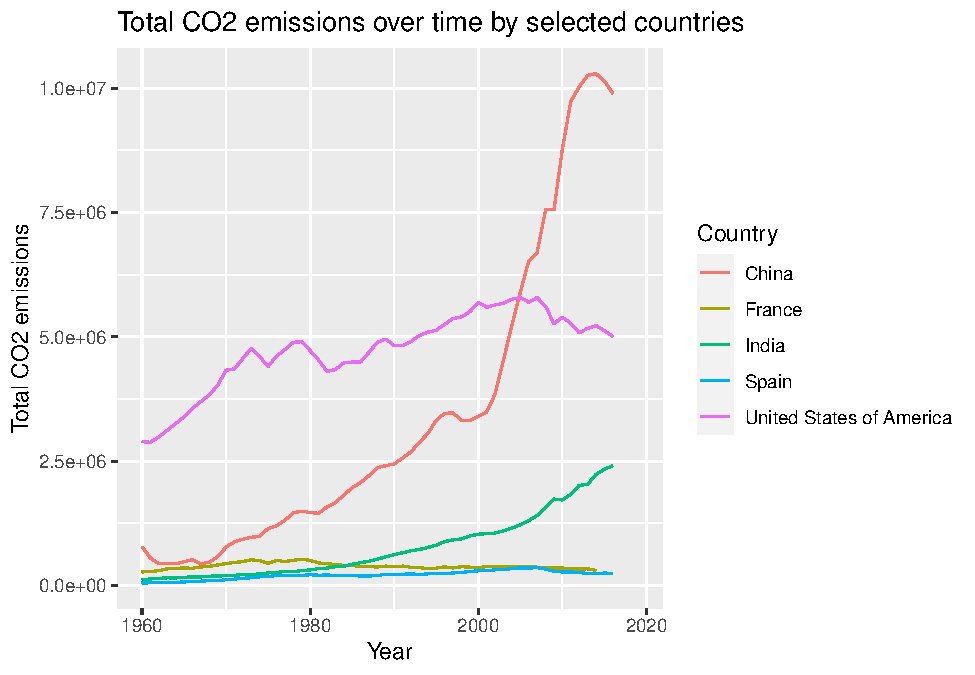
\includegraphics{ps05-rmarkdown_files/figure-latex/unnamed-chunk-9-1.pdf}
\#\#\#The plot shows that the United States and China continue to be the
top two countries with the highest CO2 emissions, with both countries'
emissions rising rapidly since the 1990s. India's CO2 emissions have
also been increasing steadily over time, though at a slower rate than
the United States and China.

\#\#3. (5pt) Now let's analyze the CO2 emissions per capita (co2\_PC ).
Make a similar plot of thesame countries. What does this figure suggest?

\begin{Shaded}
\begin{Highlighting}[]
\NormalTok{gapminder }\SpecialCharTok{\%\textgreater{}\%}
  \FunctionTok{filter}\NormalTok{(name }\SpecialCharTok{==} \StringTok{"United States of America"} \SpecialCharTok{|}\NormalTok{name }\SpecialCharTok{==} \StringTok{"China"} \SpecialCharTok{|}\NormalTok{ name }\SpecialCharTok{==} \StringTok{"India"} \SpecialCharTok{|}\NormalTok{name }\SpecialCharTok{==} \StringTok{"Spain"}\SpecialCharTok{|}\NormalTok{name }\SpecialCharTok{==} \StringTok{"France"}\NormalTok{) }\SpecialCharTok{\%\textgreater{}\%}
  \FunctionTok{select}\NormalTok{(time, co2\_PC, name) }\SpecialCharTok{\%\textgreater{}\%}
  \FunctionTok{ggplot}\NormalTok{(}\FunctionTok{aes}\NormalTok{(}\AttributeTok{x =}\NormalTok{ time, }\AttributeTok{y =}\NormalTok{ co2\_PC, }\AttributeTok{color =}\NormalTok{ name)) }\SpecialCharTok{+}
  \FunctionTok{geom\_line}\NormalTok{() }\SpecialCharTok{+}
  \FunctionTok{labs}\NormalTok{( }\AttributeTok{color =} \StringTok{"Country"}\NormalTok{, }\AttributeTok{title =} \StringTok{"CO2 emissions per capita over time by selected countries"}\NormalTok{, }\AttributeTok{x =} \StringTok{"Year"}\NormalTok{, }\AttributeTok{y =} \StringTok{"CO2 emissions per capita"}\NormalTok{)}
\end{Highlighting}
\end{Shaded}

\begin{verbatim}
## Warning: Removed 17 rows containing missing values (`geom_line()`).
\end{verbatim}

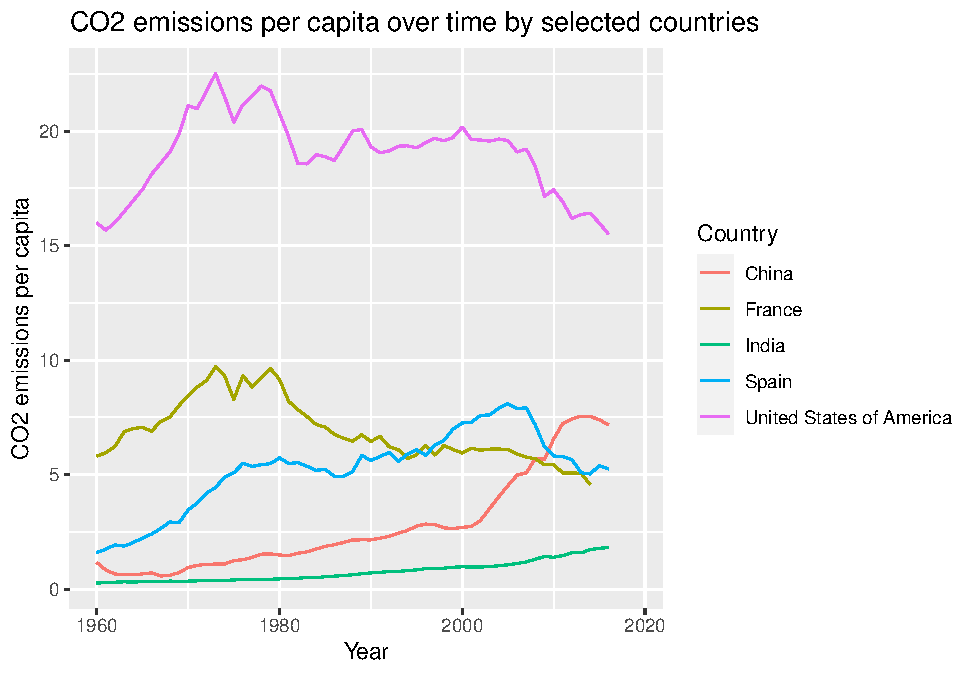
\includegraphics{ps05-rmarkdown_files/figure-latex/unnamed-chunk-10-1.pdf}
\#\#\#The plot shows that the United States has consistently had the
highest CO2 emissions per capita of the selected countries, with the
exception of a brief dip in the 1970s. China and India have had lower
CO2 emissions per capita, but both countries have experienced rapid
increases in emissions since around 2000.

\#\#4.(6pt) Compute average CO2 emissions per capita across the
continents (assume region is thesame as continent). Comment what do you
see. \#\#Note: just compute averages over countries and ignore the fact
that countries are of different size.

\begin{Shaded}
\begin{Highlighting}[]
\NormalTok{gapminder }\SpecialCharTok{\%\textgreater{}\%} 
  \FunctionTok{filter}\NormalTok{(time }\SpecialCharTok{==} \DecValTok{1960} \SpecialCharTok{|}\NormalTok{ time }\SpecialCharTok{==} \DecValTok{2016}\NormalTok{, }\SpecialCharTok{!}\FunctionTok{is.na}\NormalTok{(co2\_PC), }\SpecialCharTok{!}\FunctionTok{is.na}\NormalTok{(region)) }\SpecialCharTok{\%\textgreater{}\%}
  \FunctionTok{group\_by}\NormalTok{(time, region) }\SpecialCharTok{\%\textgreater{}\%} 
  \FunctionTok{summarize}\NormalTok{(}\AttributeTok{average\_CO2\_PC =} \FunctionTok{mean}\NormalTok{(co2\_PC, }\AttributeTok{na.rm =} \ConstantTok{TRUE}\NormalTok{), }\AttributeTok{.groups =} \StringTok{\textquotesingle{}drop\textquotesingle{}}\NormalTok{) }
\end{Highlighting}
\end{Shaded}

\begin{verbatim}
## # A tibble: 10 x 3
##     time region   average_CO2_PC
##    <dbl> <chr>             <dbl>
##  1  1960 Africa            0.291
##  2  1960 Americas          7.15 
##  3  1960 Asia              1.74 
##  4  1960 Europe            5.77 
##  5  1960 Oceania           2.73 
##  6  2016 Africa            1.20 
##  7  2016 Americas          4.80 
##  8  2016 Asia              6.47 
##  9  2016 Europe            6.64 
## 10  2016 Oceania           4.57
\end{verbatim}

\#\#\#The results show that there is a large variation in average CO2
emissions per capita across the continents over time. In 1960, the
Americas had the highest average CO2 emissions per capita, while Africa
had the lowest. By 2016, Asia had the highest average CO2 emissions per
capita, while Africa still had the lowest.

\#\#5. (7pt) Make a barplot where you show the previous results--average
CO2 emissions per capitaacross continents in 1960 and 2016.Hint: it
should look something along these lines:

\begin{Shaded}
\begin{Highlighting}[]
\NormalTok{gapminder }\SpecialCharTok{\%\textgreater{}\%}
  \FunctionTok{filter}\NormalTok{(time }\SpecialCharTok{\%in\%} \FunctionTok{c}\NormalTok{(}\DecValTok{1960}\NormalTok{, }\DecValTok{2016}\NormalTok{), }\SpecialCharTok{!}\FunctionTok{is.na}\NormalTok{(region), }\SpecialCharTok{!}\FunctionTok{is.na}\NormalTok{(co2\_PC)) }\SpecialCharTok{\%\textgreater{}\%}
  \FunctionTok{group\_by}\NormalTok{(time, region) }\SpecialCharTok{\%\textgreater{}\%}
  \FunctionTok{summarise}\NormalTok{(}\AttributeTok{avg\_co2PC =} \FunctionTok{mean}\NormalTok{(co2\_PC),}\AttributeTok{.groups =} \StringTok{\textquotesingle{}drop\textquotesingle{}}\NormalTok{) }\SpecialCharTok{\%\textgreater{}\%}
  \FunctionTok{ggplot}\NormalTok{(}\FunctionTok{aes}\NormalTok{(}\AttributeTok{x =}\NormalTok{ region, }\AttributeTok{y =}\NormalTok{ avg\_co2PC, }\AttributeTok{fill =} \FunctionTok{as.factor}\NormalTok{(time))) }\SpecialCharTok{+} 
  \FunctionTok{geom\_col}\NormalTok{(}\AttributeTok{position =} \StringTok{"dodge"}\NormalTok{) }\SpecialCharTok{+} 
  \FunctionTok{labs}\NormalTok{(}\AttributeTok{title =} \StringTok{"Average CO2 emissions per capita across continents in 1960 and 2016"}\NormalTok{, }\AttributeTok{x =} \StringTok{"Continent"}\NormalTok{, }\AttributeTok{y =} \StringTok{"CO2 emissions per capita"}\NormalTok{) }\SpecialCharTok{+}
  \FunctionTok{scale\_fill\_discrete}\NormalTok{(}\AttributeTok{name =} \StringTok{"Year"}\NormalTok{)}
\end{Highlighting}
\end{Shaded}

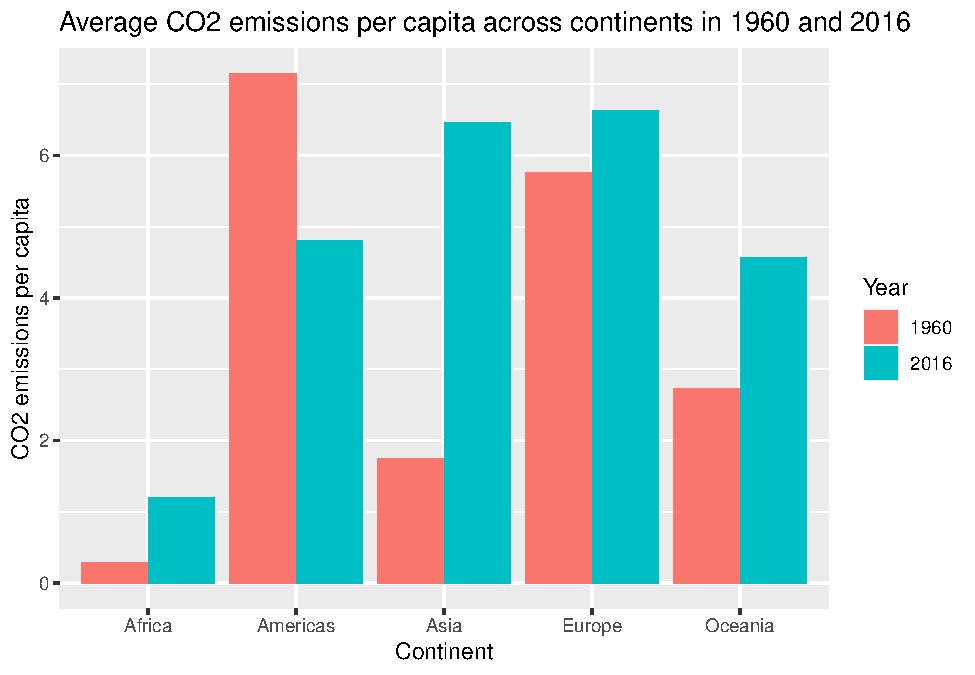
\includegraphics{ps05-rmarkdown_files/figure-latex/unnamed-chunk-12-1.pdf}
\#\#6.Which countries are the three largest, and three smallest CO2
emitters (in terms of CO2 percapita) in 2019 for each continent? (Assume
region is continent).

\begin{Shaded}
\begin{Highlighting}[]
\NormalTok{gapminder }\SpecialCharTok{\%\textgreater{}\%}
  \FunctionTok{filter}\NormalTok{(time }\SpecialCharTok{==} \DecValTok{2016}\NormalTok{, }\SpecialCharTok{!}\FunctionTok{is.na}\NormalTok{(co2\_PC), }\SpecialCharTok{!}\FunctionTok{is.na}\NormalTok{(region)) }\SpecialCharTok{\%\textgreater{}\%}
  \FunctionTok{filter}\NormalTok{(name }\SpecialCharTok{!=} \StringTok{""}\NormalTok{) }\SpecialCharTok{\%\textgreater{}\%} 
  \FunctionTok{group\_by}\NormalTok{(region, name) }\SpecialCharTok{\%\textgreater{}\%}
  \FunctionTok{summarize}\NormalTok{(}\AttributeTok{co2\_data =}\NormalTok{ co2\_PC, }\AttributeTok{.groups =} \StringTok{\textquotesingle{}drop\textquotesingle{}}\NormalTok{) }\SpecialCharTok{\%\textgreater{}\%}
  \FunctionTok{arrange}\NormalTok{(region, }\FunctionTok{desc}\NormalTok{(co2\_data)) }\SpecialCharTok{\%\textgreater{}\%}
  \FunctionTok{mutate}\NormalTok{(}\AttributeTok{ranking =} \FunctionTok{row\_number}\NormalTok{()) }\SpecialCharTok{\%\textgreater{}\%}
  \FunctionTok{filter}\NormalTok{(ranking }\SpecialCharTok{\textless{}=} \DecValTok{3} \SpecialCharTok{|}\NormalTok{ ranking }\SpecialCharTok{\textgreater{}=} \FunctionTok{n}\NormalTok{() }\SpecialCharTok{{-}} \DecValTok{2}\NormalTok{) }\SpecialCharTok{\%\textgreater{}\%}
  \FunctionTok{ungroup}\NormalTok{() }\SpecialCharTok{\%\textgreater{}\%}
  \FunctionTok{arrange}\NormalTok{(region, ranking)}
\end{Highlighting}
\end{Shaded}

\begin{verbatim}
## # A tibble: 6 x 4
##   region  name            co2_data ranking
##   <chr>   <chr>              <dbl>   <int>
## 1 Africa  South Africa       8.48        1
## 2 Africa  Libya              7.79        2
## 3 Africa  Seychelles         6.39        3
## 4 Oceania Kiribati           0.587     200
## 5 Oceania Vanuatu            0.527     201
## 6 Oceania Solomon Islands    0.272     202
\end{verbatim}

\#4 GDP per capita (50pt) \#\#Let's look at GDP per capita (GDP\_PC ).
\#\#1. (8pt) Make a scatterplot of GDP per capita versus life expectancy
by country, using data for1960. Make the point size dependent on the
country size, and color those according to thecontinent. Feel free to
adjust the plot in other ways to make it better.Comment what do you see
there.

\begin{Shaded}
\begin{Highlighting}[]
\NormalTok{gapminder }\SpecialCharTok{\%\textgreater{}\%}
  \FunctionTok{filter}\NormalTok{(time }\SpecialCharTok{==} \DecValTok{1960} \SpecialCharTok{\&} \SpecialCharTok{!}\FunctionTok{is.na}\NormalTok{(region),}
         \SpecialCharTok{!}\FunctionTok{is.na}\NormalTok{(GDP\_PC),}
         \SpecialCharTok{!}\FunctionTok{is.na}\NormalTok{(lifeExpectancy)) }\SpecialCharTok{\%\textgreater{}\%}
  \FunctionTok{ggplot}\NormalTok{(}\FunctionTok{aes}\NormalTok{(GDP\_PC, lifeExpectancy, }\AttributeTok{size =}\NormalTok{ totalPopulation, }\AttributeTok{col =}\NormalTok{ region)) }\SpecialCharTok{+}
    \FunctionTok{geom\_point}\NormalTok{() }\SpecialCharTok{+}
  \FunctionTok{labs}\NormalTok{(}\AttributeTok{title =} \StringTok{"GDP per capita vs Life expectancy by country (1960)"}\NormalTok{, }\AttributeTok{x =} \StringTok{"GDP per capita"}\NormalTok{, }\AttributeTok{y =} \StringTok{"Life expectancy at birth"}\NormalTok{)}
\end{Highlighting}
\end{Shaded}

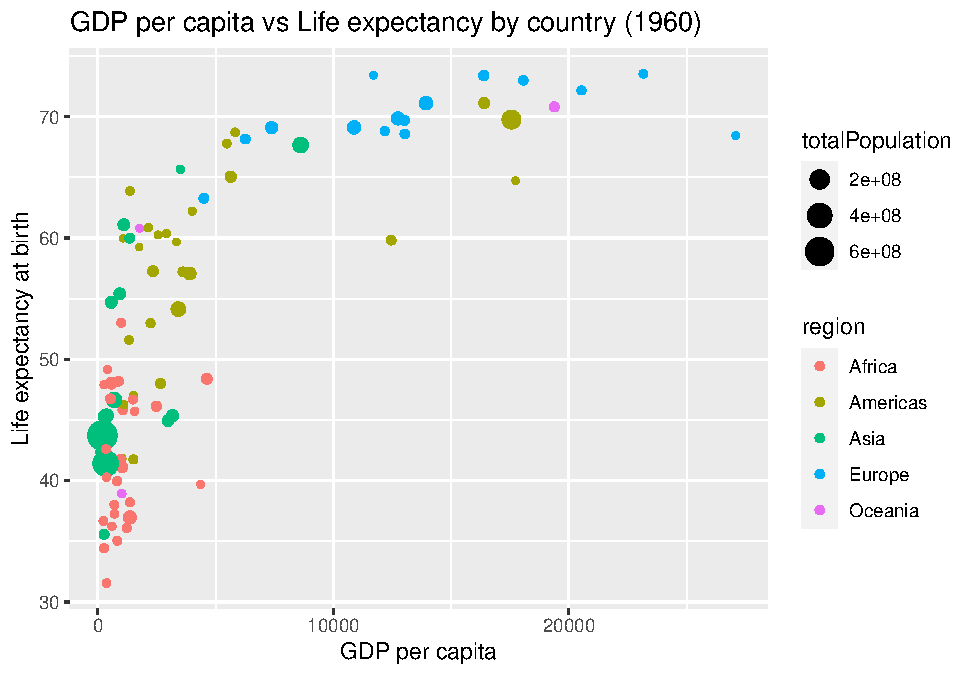
\includegraphics{ps05-rmarkdown_files/figure-latex/unnamed-chunk-14-1.pdf}
\#\#\#The plot shows that there is a positive relationship between GDP
per capita and life expectancy, with countries with higher GDP per
capita generally having higher life expectancies. However, there is a
wide variation in life expectancy within each level of GDP per capita,
suggesting that other factors besides economic development also play a
role in determining life expectancy.

\#\#2. (4pt) Make a similar plot, but this time use 2019 data only.

\begin{Shaded}
\begin{Highlighting}[]
\NormalTok{gapminder }\SpecialCharTok{\%\textgreater{}\%}
  \FunctionTok{filter}\NormalTok{(time }\SpecialCharTok{==} \DecValTok{2019} \SpecialCharTok{\&} \SpecialCharTok{!}\FunctionTok{is.na}\NormalTok{(region),}
         \SpecialCharTok{!}\FunctionTok{is.na}\NormalTok{(GDP\_PC),}
         \SpecialCharTok{!}\FunctionTok{is.na}\NormalTok{(lifeExpectancy)) }\SpecialCharTok{\%\textgreater{}\%}
  \FunctionTok{ggplot}\NormalTok{(}\FunctionTok{aes}\NormalTok{(GDP\_PC, lifeExpectancy, }\AttributeTok{size =}\NormalTok{ totalPopulation, }\AttributeTok{col =}\NormalTok{ region)) }\SpecialCharTok{+}
    \FunctionTok{geom\_point}\NormalTok{()}\SpecialCharTok{+}
  \FunctionTok{labs}\NormalTok{(}\AttributeTok{title =} \StringTok{"GDP per capita vs Life expectancy by country (2019)"}\NormalTok{, }\AttributeTok{x =} \StringTok{"GDP per capita"}\NormalTok{, }\AttributeTok{y =} \StringTok{"Life expectancy at birth"}\NormalTok{)}
\end{Highlighting}
\end{Shaded}

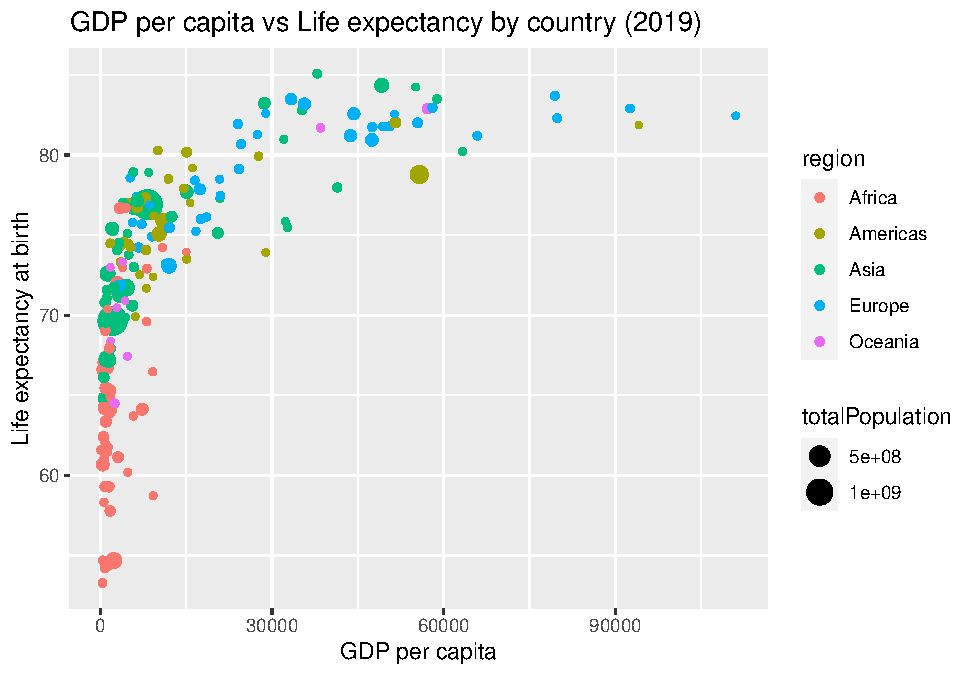
\includegraphics{ps05-rmarkdown_files/figure-latex/unnamed-chunk-15-1.pdf}
\#\#3. (6pt) Compare these two plots and comment what do you see. How
has world developed through the last 60 years?

\#\#\#The overall relationship between GDP per capita and life
expectancy remains strong for both years, with countries with higher GDP
per capita tending to have higher life expectancy. However, the
relationship appears to be stronger in 2019 than in 1960, with the
points in the upper right quadrant of the graph clustered more closely,
and the range of GDP per capita values and life expectancy increasing
substantially over the past 60 years. In 1960, most countries had per
capita GDP values below \$10,000, and life expectancy in many countries
was below 50 years. By 2019, many countries had per capita GDP values
exceeding \$10,000 and minimum life expectancy values exceeding 50
years. These last two graphs show that the world has experienced
significant economic and social development over the past 60 years, with
many countries experiencing significant improvements in GDP per capita
and life expectancy.

\#\#4. (6pt) Compute the average life expectancy for each continent in
1960 and 2019. Do the resultsfit with what do you see on the
figures?Note: here as average I mean just average over countries, ignore
the fact that countries are ofdifferent size.

\begin{Shaded}
\begin{Highlighting}[]
\FunctionTok{library}\NormalTok{(tidyverse)}
\end{Highlighting}
\end{Shaded}

\begin{verbatim}
## -- Attaching packages --------------------------------------- tidyverse 1.3.2 --
## v tibble  3.1.8     v stringr 1.5.0
## v tidyr   1.3.0     v forcats 1.0.0
## v purrr   1.0.1     
## -- Conflicts ------------------------------------------ tidyverse_conflicts() --
## x dplyr::filter() masks stats::filter()
## x dplyr::lag()    masks stats::lag()
\end{verbatim}

\begin{Shaded}
\begin{Highlighting}[]
\NormalTok{lifeexp\_continents }\OtherTok{\textless{}{-}}\NormalTok{ gapminder }\SpecialCharTok{\%\textgreater{}\%} 
  \FunctionTok{filter}\NormalTok{(time }\SpecialCharTok{\%in\%} \FunctionTok{c}\NormalTok{(}\DecValTok{1960}\NormalTok{, }\DecValTok{2019}\NormalTok{), }\SpecialCharTok{!}\FunctionTok{is.na}\NormalTok{(region)) }\SpecialCharTok{\%\textgreater{}\%} 
  \FunctionTok{group\_by}\NormalTok{(region, time) }\SpecialCharTok{\%\textgreater{}\%} 
  \FunctionTok{summarize}\NormalTok{(}\AttributeTok{avg\_life\_expectancy =} \FunctionTok{mean}\NormalTok{(lifeExpectancy, }\AttributeTok{na.rm =} \ConstantTok{TRUE}\NormalTok{), }\AttributeTok{.groups =} \StringTok{\textquotesingle{}drop\textquotesingle{}}\NormalTok{)}

\NormalTok{lifeexp\_continents\_wide }\OtherTok{\textless{}{-}} \FunctionTok{spread}\NormalTok{(lifeexp\_continents, time, avg\_life\_expectancy)}

\NormalTok{knitr}\SpecialCharTok{::}\FunctionTok{kable}\NormalTok{(lifeexp\_continents\_wide, }\AttributeTok{caption =} \StringTok{"Average life expectancy by continent and year"}\NormalTok{)}
\end{Highlighting}
\end{Shaded}

\begin{longtable}[]{@{}lrr@{}}
\caption{Average life expectancy by continent and year}\tabularnewline
\toprule()
region & 1960 & 2019 \\
\midrule()
\endfirsthead
\toprule()
region & 1960 & 2019 \\
\midrule()
\endhead
Africa & 41.46600 & 64.11014 \\
Americas & 58.64651 & 75.83206 \\
Asia & 51.64931 & 74.61739 \\
Europe & 68.28254 & 79.35714 \\
Oceania & 56.39613 & 73.52827 \\
\bottomrule()
\end{longtable}

\#\#\#The results are consistent with what we saw in the plots.

\#\#5. (8pt) Compute the average LE growth from 1960-2019 across the
continents. Show the results in the order of growth. Explain what do you
see. Hint: these data (data in long form) is not the simplest to compute
growth. But you may want to check out the lag() function. And do not
forget to group data by continent when using lag(), otherwise your
results will be messed up! See
\url{https://faculty.washington.edu/otoomet/info201-book/dplyr.html\#dplyr-helpers-compute}.

\begin{Shaded}
\begin{Highlighting}[]
\NormalTok{lifeexp\_growth }\OtherTok{\textless{}{-}}\NormalTok{ gapminder }\SpecialCharTok{\%\textgreater{}\%} 
  \FunctionTok{filter}\NormalTok{(time }\SpecialCharTok{\%in\%} \FunctionTok{c}\NormalTok{(}\DecValTok{1960}\NormalTok{, }\DecValTok{2019}\NormalTok{),}\SpecialCharTok{!}\FunctionTok{is.na}\NormalTok{(region)) }\SpecialCharTok{\%\textgreater{}\%} 
  \FunctionTok{group\_by}\NormalTok{(region) }\SpecialCharTok{\%\textgreater{}\%} 
  \FunctionTok{summarize}\NormalTok{(}\AttributeTok{avg\_life\_expectancy\_1960 =} \FunctionTok{mean}\NormalTok{(lifeExpectancy[time }\SpecialCharTok{==} \DecValTok{1960}\NormalTok{], }\AttributeTok{na.rm =} \ConstantTok{TRUE}\NormalTok{),}
            \AttributeTok{avg\_life\_expectancy\_2019 =} \FunctionTok{mean}\NormalTok{(lifeExpectancy[time }\SpecialCharTok{==} \DecValTok{2019}\NormalTok{], }\AttributeTok{na.rm =} \ConstantTok{TRUE}\NormalTok{),}
            \AttributeTok{life\_expectancy\_growth =}\NormalTok{ avg\_life\_expectancy\_2019 }\SpecialCharTok{{-}}\NormalTok{ avg\_life\_expectancy\_1960,}
            \AttributeTok{growth\_rate =}\NormalTok{ ((avg\_life\_expectancy\_2019 }\SpecialCharTok{/}\NormalTok{ avg\_life\_expectancy\_1960) }\SpecialCharTok{\^{}}\NormalTok{ (}\DecValTok{1} \SpecialCharTok{/} \DecValTok{59}\NormalTok{)) }\SpecialCharTok{{-}} \DecValTok{1}\NormalTok{) }\SpecialCharTok{\%\textgreater{}\%} 
  \FunctionTok{arrange}\NormalTok{(life\_expectancy\_growth)}

\NormalTok{knitr}\SpecialCharTok{::}\FunctionTok{kable}\NormalTok{(lifeexp\_growth, }\AttributeTok{caption =} \StringTok{"Average LE growth from 1960 to 2019 by continent"}\NormalTok{)}
\end{Highlighting}
\end{Shaded}

\begin{longtable}[]{@{}
  >{\raggedright\arraybackslash}p{(\columnwidth - 8\tabcolsep) * \real{0.0957}}
  >{\raggedleft\arraybackslash}p{(\columnwidth - 8\tabcolsep) * \real{0.2660}}
  >{\raggedleft\arraybackslash}p{(\columnwidth - 8\tabcolsep) * \real{0.2660}}
  >{\raggedleft\arraybackslash}p{(\columnwidth - 8\tabcolsep) * \real{0.2447}}
  >{\raggedleft\arraybackslash}p{(\columnwidth - 8\tabcolsep) * \real{0.1277}}@{}}
\caption{Average LE growth from 1960 to 2019 by
continent}\tabularnewline
\toprule()
\begin{minipage}[b]{\linewidth}\raggedright
region
\end{minipage} & \begin{minipage}[b]{\linewidth}\raggedleft
avg\_life\_expectancy\_1960
\end{minipage} & \begin{minipage}[b]{\linewidth}\raggedleft
avg\_life\_expectancy\_2019
\end{minipage} & \begin{minipage}[b]{\linewidth}\raggedleft
life\_expectancy\_growth
\end{minipage} & \begin{minipage}[b]{\linewidth}\raggedleft
growth\_rate
\end{minipage} \\
\midrule()
\endfirsthead
\toprule()
\begin{minipage}[b]{\linewidth}\raggedright
region
\end{minipage} & \begin{minipage}[b]{\linewidth}\raggedleft
avg\_life\_expectancy\_1960
\end{minipage} & \begin{minipage}[b]{\linewidth}\raggedleft
avg\_life\_expectancy\_2019
\end{minipage} & \begin{minipage}[b]{\linewidth}\raggedleft
life\_expectancy\_growth
\end{minipage} & \begin{minipage}[b]{\linewidth}\raggedleft
growth\_rate
\end{minipage} \\
\midrule()
\endhead
Europe & 68.28254 & 79.35714 & 11.07460 & 0.0025508 \\
Oceania & 56.39613 & 73.52827 & 17.13214 & 0.0045062 \\
Americas & 58.64651 & 75.83206 & 17.18555 & 0.0043653 \\
Africa & 41.46600 & 64.11014 & 22.64414 & 0.0074126 \\
Asia & 51.64931 & 74.61739 & 22.96808 & 0.0062550 \\
\bottomrule()
\end{longtable}

\#\#\#The average life expectancy has increased for all continents from
1960 to 2019. The average growth rate for life expectancy is highest for
Africa, followed by Oceania, the Americas, Asia, and Europe.

\#\#6. (6pt) Show the histogram of GDP per capita for years of 1960 and
2019. Try to put both histograms on the same graph, see how well you can
do it!

\begin{Shaded}
\begin{Highlighting}[]
\NormalTok{gapminder }\SpecialCharTok{\%\textgreater{}\%}
  \FunctionTok{filter}\NormalTok{(time }\SpecialCharTok{==} \DecValTok{1960} \SpecialCharTok{|}\NormalTok{ time }\SpecialCharTok{==} \DecValTok{2019}\NormalTok{,}
         \SpecialCharTok{!}\FunctionTok{is.na}\NormalTok{(GDP\_PC)) }\SpecialCharTok{\%\textgreater{}\%}
  \FunctionTok{ggplot}\NormalTok{(}\FunctionTok{aes}\NormalTok{(GDP\_PC, }\AttributeTok{fill =} \FunctionTok{factor}\NormalTok{(time))) }\SpecialCharTok{+}
  \FunctionTok{geom\_histogram}\NormalTok{(}\AttributeTok{position =} \StringTok{"dodge"}\NormalTok{, }\AttributeTok{bins =} \DecValTok{8}\NormalTok{) }\SpecialCharTok{+}
  \FunctionTok{labs}\NormalTok{(}\AttributeTok{title =} \StringTok{"Distribution of GDP per capita by year"}\NormalTok{, }\AttributeTok{x =} \StringTok{"GDP per capita"}\NormalTok{, }\AttributeTok{y =} \StringTok{"Frequency"}\NormalTok{) }
\end{Highlighting}
\end{Shaded}

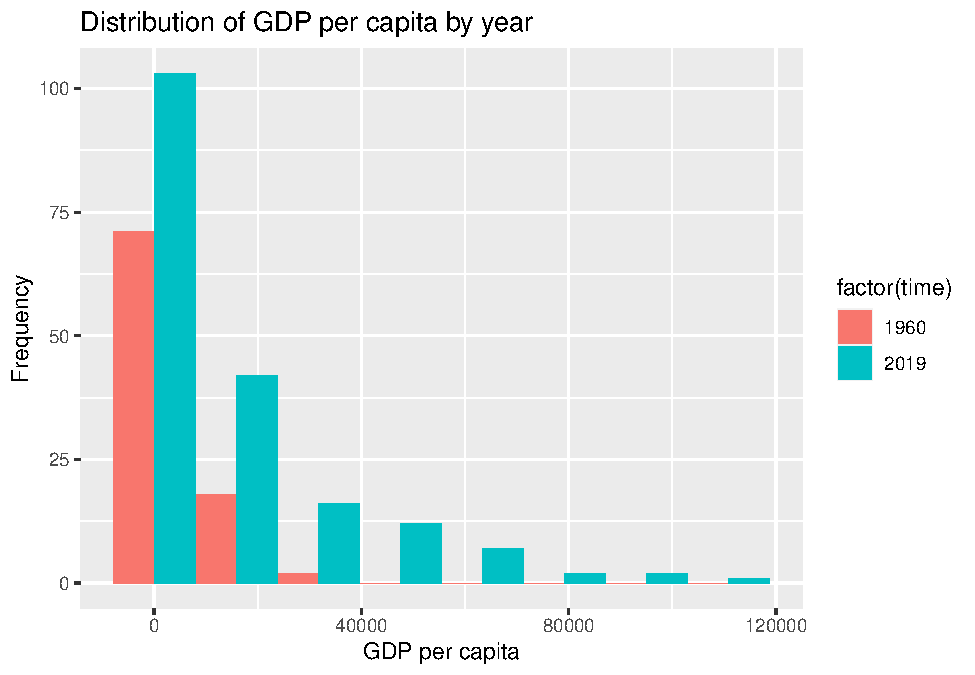
\includegraphics{ps05-rmarkdown_files/figure-latex/unnamed-chunk-18-1.pdf}
\#\#7. (6pt) What was the ranking of US in terms of life expectancy in
1960 and in 2019? (When counting from top.) Hint: check out the function
rank()! Hint2: 17 for 1960.

\begin{Shaded}
\begin{Highlighting}[]
\NormalTok{gapminder }\SpecialCharTok{\%\textgreater{}\%}
  \FunctionTok{filter}\NormalTok{(time }\SpecialCharTok{==} \DecValTok{1960} \SpecialCharTok{|}\NormalTok{ time }\SpecialCharTok{==} \DecValTok{2019}\NormalTok{,}
         \SpecialCharTok{!}\FunctionTok{is.na}\NormalTok{(name)) }\SpecialCharTok{\%\textgreater{}\%}
  \FunctionTok{group\_by}\NormalTok{(time) }\SpecialCharTok{\%\textgreater{}\%}
  \FunctionTok{mutate}\NormalTok{(}\AttributeTok{rank =} \FunctionTok{rank}\NormalTok{(}\FunctionTok{desc}\NormalTok{(lifeExpectancy))) }\SpecialCharTok{\%\textgreater{}\%}
  \FunctionTok{filter}\NormalTok{(iso3 }\SpecialCharTok{==} \StringTok{"USA"}\NormalTok{) }\SpecialCharTok{\%\textgreater{}\%}
  \FunctionTok{select}\NormalTok{(name, time, lifeExpectancy, rank) }\SpecialCharTok{\%\textgreater{}\%}
  \FunctionTok{print}\NormalTok{()}
\end{Highlighting}
\end{Shaded}

\begin{verbatim}
## # A tibble: 2 x 4
## # Groups:   time [2]
##   name                      time lifeExpectancy  rank
##   <chr>                    <dbl>          <dbl> <dbl>
## 1 United States of America  1960           69.8    17
## 2 United States of America  2019           78.8    46
\end{verbatim}

\#\#8. (6pt) If you did this correctly, then you noticed that US ranking
has been falling quite a bit. But we also have more countries in
2019--what about the relative rank divided by the corresponding number
of countries that have LE data in the corresponding year? Hint: 0.0904
for 1960.

\begin{Shaded}
\begin{Highlighting}[]
\NormalTok{gapminder }\SpecialCharTok{\%\textgreater{}\%}
  \FunctionTok{filter}\NormalTok{(time }\SpecialCharTok{==} \DecValTok{1960} \SpecialCharTok{|}\NormalTok{ time }\SpecialCharTok{==} \DecValTok{2019}\NormalTok{,}
         \SpecialCharTok{!}\FunctionTok{is.na}\NormalTok{(name) }\SpecialCharTok{\&} \SpecialCharTok{!}\FunctionTok{is.na}\NormalTok{(lifeExpectancy)) }\SpecialCharTok{\%\textgreater{}\%}
  \FunctionTok{group\_by}\NormalTok{(time) }\SpecialCharTok{\%\textgreater{}\%}
  \FunctionTok{mutate}\NormalTok{(}\AttributeTok{ranking =} \FunctionTok{rank}\NormalTok{(}\FunctionTok{desc}\NormalTok{(lifeExpectancy))) }\SpecialCharTok{\%\textgreater{}\%}
  \FunctionTok{mutate}\NormalTok{(}\AttributeTok{perc =}\NormalTok{ ranking }\SpecialCharTok{/} \FunctionTok{n}\NormalTok{()) }\SpecialCharTok{\%\textgreater{}\%}
  \FunctionTok{filter}\NormalTok{(iso3 }\SpecialCharTok{==} \StringTok{"USA"}\NormalTok{) }\SpecialCharTok{\%\textgreater{}\%}
  \FunctionTok{select}\NormalTok{(name, time, ranking, perc) }
\end{Highlighting}
\end{Shaded}

\begin{verbatim}
## # A tibble: 2 x 4
## # Groups:   time [2]
##   name                      time ranking   perc
##   <chr>                    <dbl>   <dbl>  <dbl>
## 1 United States of America  1960      17 0.0904
## 2 United States of America  2019      46 0.235
\end{verbatim}

\#\#Finally tell us how many hours did you spend on this PS. \#\#\#
10hours

\end{document}
